\section{Results}\label{sec:results}
The results of all the 192 experiments on Arabic dataset and the 192 experiments on the English
dataset are presented and discussed; for each dataset, we start with the overall accuracy
followed by the individual accuracy on each class (meter).


\subsection{Results of Arabic dataset}\label{sec:arabic-results}
\subsubsection{Overall Accuracy}\label{sec:encoding-effect}
\begin{figure}[!tb]
  \centering
  \begin{tikzpicture}[scale=0.90]

  %% two grid to help during positioning.
  % \draw[step=0.2, green!40, thin] (0,0) grid (8,6);
  % \draw[step=1, red!40, very thin] (0,-1) grid (8,7);

  %% Variables
  \def \maxHeight{5.7}
  \def \yONE{-0.8}
  \def \yTWO{-0.3}

  %% two colored areas to distinguish the diacritic models.
  \fill[gray!30, opacity=0.2, rounded corners=2pt] (0,-0.5) rectangle (2.1,\maxHeight);
  \fill[gray!30, opacity=0.2, rounded corners=2pt] (4.2,-0.5) rectangle (6.32,\maxHeight);

  %% The Full/Eliminated Vertical Separating line.
  \draw[dashed, thick] (4.2, 0 - 0.9) -- (4.2, \maxHeight +0.5);

  %% Group Labels Full/Eliminated
  \node [align=center, text width=3cm, inner sep=0.25cm] at (2.1, \yONE) {\scriptsize no trimming(0T)};
  \node [align=center, text width=4cm, inner sep=0.25cm] at (6.32,\yONE) {\scriptsize trimming(1T)};

  \node [align=center, text width=3cm, inner sep=0.25cm] at (1, \yTWO) {\scriptsize diacritic(1D)};
  \node [align=center, text width=3cm, inner sep=0.25cm] at (3, \yTWO) {\scriptsize no diacritic(0D)};
  \node [align=center, text width=3cm, inner sep=0.25cm] at (5+0.2, \yTWO) {\scriptsize diacritic(1D)};
  \node [align=center, text width=3cm, inner sep=0.25cm] at (7+0.2, \yTWO) {\scriptsize no diacritic(0D)};

  % Points annotations
  \def \layerHeight{5.7}
  \def \unitHeight{\layerHeight - 0.3}
  \def \weightedHeihgt{\layerHeight - 0.6}

  \def \step{0.2}
  \def \move{0.1}
  %%%%%% 

  \node  at (3.5*   \step -0.15-\move, \layerHeight) {\scriptsize 7L};
  \node  at (3.5*   \step -0.15-\move, \unitHeight) {\scriptsize 82U};
  \node  at (3.5*   \step -0.1 -\move, \weightedHeihgt) {\scriptsize 0};

  \node  at (5.2*   \step, \layerHeight) {\scriptsize 7L};
  \node  at (5.2*   \step, \unitHeight) {\scriptsize 50U};
  \node  at (5.2*   \step, \weightedHeihgt) {\scriptsize 1};

  \node  at (7*     \step +0.15+\move, \layerHeight) {\scriptsize 7L};
  \node  at (7*   \step   +0.15+\move, \unitHeight) {\scriptsize 50U};
  \node  at (7*   \step   +0.1 +\move, \weightedHeihgt) {\scriptsize 1};

  %%%%%%

  \node  at (14*    \step -0.15-\move, \layerHeight) {\scriptsize 7L};
  \node  at (14*   \step -0.15 -\move, \unitHeight) {\scriptsize 82U};
  \node  at (14*   \step -0.1  -\move, \weightedHeihgt) {\scriptsize 0};

  \node  at (16*    \step, \layerHeight) {\scriptsize 7L};
  \node  at (16*    \step, \unitHeight) {\scriptsize 82U};
  \node  at (16*    \step, \weightedHeihgt) {\scriptsize 0};

  \node  at (17.6*  \step +0.15+\move, \layerHeight) {\scriptsize 7L};
  \node  at (17.6*  \step +0.15+\move, \unitHeight) {\scriptsize 50U};
  \node  at (17.6*  \step +0.1 +\move, \weightedHeihgt) {\scriptsize 0};

  %%%%%%

  \node  at (24.5*  \step -0.15-\move, \layerHeight) {\scriptsize 7L};
  \node  at (24.5*  \step -0.15-\move, \unitHeight) {\scriptsize 82U};
  \node  at (24.5*  \step -0.1 -\move,  \weightedHeihgt) {\scriptsize 1};

  \node  at (26.1*  \step, \layerHeight) {\scriptsize 7L};
  \node  at (26.1*  \step, \unitHeight) {\scriptsize 82U};
  \node  at (26.1*  \step, \weightedHeihgt) {\scriptsize 0};

  \node  at (28*    \step +0.15+\move, \layerHeight) {\scriptsize 7L};
  \node  at (28*    \step +0.15+\move, \unitHeight) {\scriptsize 82U};
  \node  at (28*    \step +0.1 +\move,  \weightedHeihgt) {\scriptsize 1};

  %%%%%%

  \node  at (35*    \step -0.15-\move, \layerHeight) {\scriptsize 4L};
  \node  at (35*    \step -0.15-\move, \unitHeight) {\scriptsize 82U};
  \node  at (35*    \step -0.1 -\move,  \weightedHeihgt) {\scriptsize 0};

  \node  at (37*    \step, \layerHeight) {\scriptsize 7L};
  \node  at (37*    \step, \unitHeight) {\scriptsize 82U};
  \node  at (37*    \step, \weightedHeihgt) {\scriptsize 0};

  \node  at (38.7*  \step +0.15+\move, \layerHeight) {\scriptsize 4L};
  \node  at (38.7*  \step +0.15+\move, \unitHeight) {\scriptsize 50U};
  \node  at (38.7*  \step +0.1 +\move,  \weightedHeihgt) {\scriptsize 1};

  \begin{axis}[
    major x tick style = transparent,
    ybar=2*\pgflinewidth,
    x=10pt,
    ymajorgrids = true,
    ylabel = {Accuracy},
    ylabel style = {font=\footnotesize},
    xtickmin={1},
    xtickmax={21},
    axis x line = bottom,
    axis y line = left,
    enlarge y limits={upper, value=0.1},
    xticklabels = {,,},
    bar shift=0pt,
    enlarge x limits=0.1,
    ymin=0.76,
    ymax=0.98,
    legend style={at={(0.5, -0.4)}, anchor=north, legend columns=3},
    every axis legend/.append style={nodes={right}},
    nodes near coords={\vspace*{0.1\baselineskip}
      \foreach \X in \pgfplotspointmeta%
      {\centerline{\X}\newline}%
      \vspace*{-0.7\baselineskip}
    },
    nodes near coords style={font=\scriptsize,anchor=-90, text width=1cm},
    ]


    % Binary
    \addplot[pointBiLSTM=blue] coordinates {

    % BLSTM
    (1, 0.9025442765600247)  % Exp_7_T1_D1_binary_BLSTM_6_82_0
    (7, 0.8766640656404435)  % Exp_7_T1_D0_binary_BLSTM_6_82_0
    (13, 0.8988593838876747) % Exp_8_T0_D1_binary_BLSTM_6_82_1
    (19, 0.9638475586025206) % Exp_3_T0_D0_binary_BLSTM_3_82_0
    };

    % Binary
    \addplot[pointLSTM=blue] coordinates {
    % LSTM
    (1, 0.7977761225792721) % Exp_11_T1_D1_binary_LSTM_3_82_0
    (7, 0.7883237568276937) % Exp_13_T1_D0_binary_LSTM_6_50_0
    (13, 0.827841810615813) % Exp_15_T0_D1_binary_LSTM_6_82_0
    (19, 0.816387749603329) % Exp_12_T0_D0_binary_LSTM_3_82_1
    };

    % OneHot
    \addplot[pointBiLSTM=red] coordinates {
    (2, 0.9346846846846846)  % Exp_6_T1_D1_onehot_BLSTM_6_50_1
    (8, 0.9310432479723819)  % Exp_7_T1_D0_onehot_BLSTM_6_82_0
    (14, 0.9472562344699578) % Exp_7_T0_D1_onehot_BLSTM_6_82_0
    (20, 0.9280962787773555) % Exp_7_T0_D0_onehot_BLSTM_6_82_0
    };

    % OneHot
    \addplot[pointLSTM=red] coordinates {
    (2, 0.8965678276701898)  % Exp_11_T1_D1_onehot_LSTM_3_82_0
    (8, 0.8869854106074577)  % Exp_9_T1_D0_onehot_LSTM_3_50_0
    (14, 0.9094811843247613) % Exp_12_T0_D1_onehot_LSTM_3_82_1
    (20, 0.9219171930664911) % Exp_15_T0_D0_onehot_LSTM_6_82_0
    };

    % TwoHot
    \addplot[pointBiLSTM=brown] coordinates {
    (3, 0.9458158946347922) % Exp_6_T1_D1_twohot_BLSTM_6_50_1
    (9, 0.9411340474332599) % Exp_5_T1_D0_twohot_BLSTM_6_50_0
    (15, 0.954692692273149) % Exp_8_T0_D1_twohot_BLSTM_6_82_1
    (21, 0.9628835733317367) % Exp_2_T0_D0_twohot_BLSTM_3_50_1
    };

    % TwoHowt
    \addplot[pointLSTM=brown] coordinates {
    (3, 0.9170331749071906)  % Exp_12_T1_D1_twohot_LSTM_3_82_1
    (9, 0.8972239956491926)  % Exp_9_T1_D0_twohot_LSTM_3_50_0
    (15, 0.94120887345448)   % Exp_11_T0_D1_twohot_LSTM_3_82_0
    (21, 0.9284854653773613) % Exp_12_T0_D0_twohot_LSTM_3_82_1
    };




    %%%%%%%%%%%%%%%%%%%%%
    %% The rest models
    %%%%%%%%%%%%%%%%%%%%%
    % Binary
    \addplot[pointRug=blue, mark size=0.7pt]
    coordinates {
      % 1, 7, 13, 19

%
(1, 0.861495353621338)  % Exp_2_T1_D1_binary_BLSTM_3_50_1
(1, 0.866862925918044)  % Exp_4_T1_D1_binary_BLSTM_3_82_1
(1, 0.867725993710246)  % Exp_1_T1_D1_binary_BLSTM_3_50_0
(1, 0.8706225910950319) % Exp_5_T1_D1_binary_BLSTM_6_50_0
(1, 0.8794601688302476) % Exp_6_T1_D1_binary_BLSTM_6_50_1
(1, 0.8869558534912864) % Exp_3_T1_D1_binary_BLSTM_3_82_0
(1, 0.8948003121231469) % Exp_8_T1_D1_binary_BLSTM_6_82_1
(1, 0.9025442765600247) % Exp_7_T1_D1_binary_BLSTM_6_82_0

(1, 0.23921165259747937) % Exp_10_T1_D1_binary_LSTM_3_50_1
(1, 0.23921165259747937) % Exp_12_T1_D1_binary_LSTM_3_82_1
(1, 0.23921165259747937) % Exp_13_T1_D1_binary_LSTM_6_50_0
(1, 0.23921165259747937) % Exp_15_T1_D1_binary_LSTM_6_82_0
(1, 0.5386134165661725)  % Exp_16_T1_D1_binary_LSTM_6_82_1
(1, 0.6374642358894328)  % Exp_9_T1_D1_binary_LSTM_3_50_0
(1, 0.6666016410110899)  % Exp_14_T1_D1_binary_LSTM_6_50_1
(1, 0.7977761225792721)  % Exp_11_T1_D1_binary_LSTM_3_82_0

%
(7, 0.7722328627840438) % Exp_2_T1_D0_binary_BLSTM_3_50_1
(7, 0.7918174079591402) % Exp_6_T1_D0_binary_BLSTM_6_50_1
(7, 0.7977524768863351) % Exp_1_T1_D0_binary_BLSTM_3_50_0
(7, 0.8173251992149632) % Exp_5_T1_D0_binary_BLSTM_6_50_0
(7, 0.8267420964271357) % Exp_4_T1_D0_binary_BLSTM_3_82_1
(7, 0.8307795984961339) % Exp_8_T1_D0_binary_BLSTM_6_82_1
(7, 0.8564115296398761) % Exp_3_T1_D0_binary_BLSTM_3_82_0
(7, 0.8766640656404435) % Exp_7_T1_D0_binary_BLSTM_6_82_0


(7, 0.23921165259747937) % Exp_10_T1_D0_binary_LSTM_3_50_1
(7, 0.23921165259747937) % Exp_12_T1_D0_binary_LSTM_3_82_1
(7, 0.23921165259747937) % Exp_15_T1_D0_binary_LSTM_6_82_0
(7, 0.5082878153744296)  % Exp_14_T1_D0_binary_LSTM_6_50_1
(7, 0.7268331323449435)  % Exp_11_T1_D0_binary_LSTM_3_82_0
(7, 0.7272055520087017)  % Exp_9_T1_D0_binary_LSTM_3_50_0
(7, 0.7346362110141638)  % Exp_16_T1_D0_binary_LSTM_6_82_1
(7, 0.7883237568276937)  % Exp_13_T1_D0_binary_LSTM_6_50_0

%
(13, 0.8288896206927522) % Exp_1_T0_D1_binary_BLSTM_3_50_0
(13, 0.8555698589947012) % Exp_4_T0_D1_binary_BLSTM_3_82_1
(13, 0.8634134658563603) % Exp_2_T0_D1_binary_BLSTM_3_50_1
(13, 0.8649043499086908) % Exp_3_T0_D1_binary_BLSTM_3_82_0
(13, 0.8741370535580637) % Exp_6_T0_D1_binary_BLSTM_6_50_1
(13, 0.8841181929766787) % Exp_7_T0_D1_binary_BLSTM_6_82_0
(13, 0.8986558093584409) % Exp_5_T0_D1_binary_BLSTM_6_50_0
(13, 0.8988593838876747) % Exp_8_T0_D1_binary_BLSTM_6_82_1

(13, 0.6457563691883963) % Exp_10_T0_D1_binary_LSTM_3_50_1
(13, 0.740628087297548)  % Exp_13_T0_D1_binary_LSTM_6_50_0
(13, 0.7581235218393557) % Exp_16_T0_D1_binary_LSTM_6_82_1
(13, 0.7709068047780139) % Exp_11_T0_D1_binary_LSTM_3_82_0
(13, 0.7879471903721222) % Exp_9_T0_D1_binary_LSTM_3_50_0
(13, 0.8079693440708917) % Exp_14_T0_D1_binary_LSTM_6_50_1
(13, 0.8203873903541598) % Exp_12_T0_D1_binary_LSTM_3_82_1
(13, 0.827841810615813)  % Exp_15_T0_D1_binary_LSTM_6_82_0

%
(19, 0.8182558452833578) % Exp_8_T0_D0_binary_BLSTM_6_82_1
(19, 0.955668652516241) % Exp_5_T0_D0_binary_BLSTM_6_50_0
(19, 0.9576864353501182) % Exp_2_T0_D0_binary_BLSTM_3_50_1
(19, 0.9604047540640063) % Exp_1_T0_D0_binary_BLSTM_3_50_0
(19, 0.9611891147501722) % Exp_4_T0_D0_binary_BLSTM_3_82_1
(19, 0.9619555129778763) % Exp_7_T0_D0_binary_BLSTM_6_82_0
(19, 0.9621052001317247) % Exp_6_T0_D0_binary_BLSTM_6_50_1
(19, 0.9638475586025206) % Exp_3_T0_D0_binary_BLSTM_3_82_0

(19, 0.6293147322096817) % Exp_14_T0_D0_binary_LSTM_6_50_1
(19, 0.6499715594407689) % Exp_13_T0_D0_binary_LSTM_6_50_0
(19, 0.686908361524414)  % Exp_9_T0_D0_binary_LSTM_3_50_0
(19, 0.7040744843277551) % Exp_10_T0_D0_binary_LSTM_3_50_1
(19, 0.7495314792084542) % Exp_16_T0_D0_binary_LSTM_6_82_1
(19, 0.7611831272640182) % Exp_15_T0_D0_binary_LSTM_6_82_0
(19, 0.783803849953597)  % Exp_11_T0_D0_binary_LSTM_3_82_0
(19, 0.816387749603329)  % Exp_12_T0_D0_binary_LSTM_3_82_1
    };

    % OneHot
    \addplot[pointRug=red, mark size=0.7pt]
    coordinates {
      % 2, 8, 14, 20
%
(2, 0.23921165259747937) % Exp_7_T1_D1_onehot_BLSTM_6_82_0
(2, 0.23921165259747937) % Exp_8_T1_D1_onehot_BLSTM_6_82_1
(2, 0.9222411387765719)  % Exp_1_T1_D1_onehot_BLSTM_3_50_0
(2, 0.9248953678087536)  % Exp_2_T1_D1_onehot_BLSTM_3_50_1
(2, 0.9309841337400391)  % Exp_3_T1_D1_onehot_BLSTM_3_82_0
(2, 0.9320954813080796)  % Exp_4_T1_D1_onehot_BLSTM_3_82_1
(2, 0.9336324513489865)  % Exp_5_T1_D1_onehot_BLSTM_6_50_0
(2, 0.9346846846846846)  % Exp_6_T1_D1_onehot_BLSTM_6_50_1

(2, 0.23921165259747937) % Exp_12_T1_D1_onehot_LSTM_3_82_1
(2, 0.23921165259747937) % Exp_13_T1_D1_onehot_LSTM_6_50_0
(2, 0.23921165259747937) % Exp_14_T1_D1_onehot_LSTM_6_50_1
(2, 0.23921165259747937) % Exp_15_T1_D1_onehot_LSTM_6_82_0
(2, 0.23921165259747937) % Exp_16_T1_D1_onehot_LSTM_6_82_1
(2, 0.23921165259747937) % Exp_9_T1_D1_onehot_LSTM_3_50_0
(2, 0.8536213378733064)  % Exp_10_T1_D1_onehot_LSTM_3_50_1
(2, 0.8965678276701898)  % Exp_11_T1_D1_onehot_LSTM_3_82_0


%
(8, 0.23921165259747937) % Exp_5_T1_D0_onehot_BLSTM_6_50_0
(8, 0.23921165259747937) % Exp_6_T1_D0_onehot_BLSTM_6_50_1
(8, 0.9026743278711783)  % Exp_2_T1_D0_onehot_BLSTM_3_50_1
(8, 0.9032713816178385)  % Exp_1_T1_D0_onehot_BLSTM_3_50_0
(8, 0.914609491381145)   % Exp_4_T1_D0_onehot_BLSTM_3_82_1
(8, 0.9212184625570452)  % Exp_3_T1_D0_onehot_BLSTM_3_82_0
(8, 0.9275673311106383)  % Exp_8_T1_D0_onehot_BLSTM_6_82_1
(8, 0.9310432479723819)  % Exp_7_T1_D0_onehot_BLSTM_6_82_0

(8, 0.23921165259747937) % Exp_10_T1_D0_onehot_LSTM_3_50_1
(8, 0.23921165259747937) % Exp_11_T1_D0_onehot_LSTM_3_82_0
(8, 0.23921165259747937) % Exp_12_T1_D0_onehot_LSTM_3_82_1
(8, 0.23921165259747937) % Exp_13_T1_D0_onehot_LSTM_6_50_0
(8, 0.23921165259747937) % Exp_14_T1_D0_onehot_LSTM_6_50_1
(8, 0.23921165259747937) % Exp_15_T1_D0_onehot_LSTM_6_82_0
(8, 0.23921165259747937) % Exp_16_T1_D0_onehot_LSTM_6_82_1
(8, 0.8869854106074577)  % Exp_9_T1_D0_onehot_LSTM_3_50_0



%
(14, 0.24334939975451306) % Exp_8_T0_D1_onehot_BLSTM_6_82_1
(14, 0.9330898422297398)  % Exp_1_T0_D1_onehot_BLSTM_3_50_0
(14, 0.9334371164266682)  % Exp_2_T0_D1_onehot_BLSTM_3_50_1
(14, 0.9352632997036194)  % Exp_3_T0_D1_onehot_BLSTM_3_82_0
(14, 0.9392928778852199)  % Exp_4_T0_D1_onehot_BLSTM_3_82_1
(14, 0.9400592761129241)  % Exp_5_T0_D1_onehot_BLSTM_6_50_0
(14, 0.9401011885160016)  % Exp_6_T0_D1_onehot_BLSTM_6_50_1
(14, 0.9472562344699578)  % Exp_7_T0_D1_onehot_BLSTM_6_82_0

(14, 0.24334939975451306) % Exp_11_T0_D1_onehot_LSTM_3_82_0
(14, 0.24334939975451306) % Exp_13_T0_D1_onehot_LSTM_6_50_0
(14, 0.24334939975451306) % Exp_14_T0_D1_onehot_LSTM_6_50_1
(14, 0.24334939975451306) % Exp_15_T0_D1_onehot_LSTM_6_82_0
(14, 0.24334939975451306) % Exp_16_T0_D1_onehot_LSTM_6_82_1
(14, 0.24431937251145108) % Exp_10_T0_D1_onehot_LSTM_3_50_1
(14, 0.8778253450288898)  % Exp_9_T0_D1_onehot_LSTM_3_50_0
(14, 0.9094811843247613)  % Exp_12_T0_D1_onehot_LSTM_3_82_1

%
(20, 0.24334939975451306) % Exp_8_T0_D0_onehot_BLSTM_6_82_1
(20, 0.9012124659461724)  % Exp_1_T0_D0_onehot_BLSTM_3_50_0
(20, 0.9170373918510313)  % Exp_2_T0_D0_onehot_BLSTM_3_50_1
(20, 0.9248031613926893)  % Exp_5_T0_D0_onehot_BLSTM_6_50_0
(20, 0.9251264856450019)  % Exp_3_T0_D0_onehot_BLSTM_3_82_0
(20, 0.926371882765021)   % Exp_4_T0_D0_onehot_BLSTM_3_82_1
(20, 0.9275933299404245)  % Exp_6_T0_D0_onehot_BLSTM_6_50_1
(20, 0.9280962787773555)  % Exp_7_T0_D0_onehot_BLSTM_6_82_0

(20, 0.24334939975451306) % Exp_11_T0_D0_onehot_LSTM_3_82_0
(20, 0.24334939975451306) % Exp_13_T0_D0_onehot_LSTM_6_50_0
(20, 0.24334939975451306) % Exp_14_T0_D0_onehot_LSTM_6_50_1
(20, 0.24334939975451306) % Exp_9_T0_D0_onehot_LSTM_3_50_0
(20, 0.8890099691644463)  % Exp_10_T0_D0_onehot_LSTM_3_50_1
(20, 0.9013202406969434)  % Exp_12_T0_D0_onehot_LSTM_3_82_1
(20, 0.910774481334012)   % Exp_16_T0_D0_onehot_LSTM_6_82_1
(20, 0.9219171930664911)  % Exp_15_T0_D0_onehot_LSTM_6_82_0

    };
    % TwoHot
    \addplot[pointRug=brown, mark size=0.7pt]
    coordinates {
      % 3, 9, 15, 21


%
(3, 0.23921165259747937) % Exp_8_T1_D1_twohot_BLSTM_6_82_1
(3, 0.9363812631529167)  % Exp_2_T1_D1_twohot_BLSTM_3_50_1
(3, 0.9417192783334514)  % Exp_7_T1_D1_twohot_BLSTM_6_82_0
(3, 0.9424582062377337)  % Exp_3_T1_D1_twohot_BLSTM_3_82_0
(3, 0.9427892459388522)  % Exp_5_T1_D1_twohot_BLSTM_6_50_0
(3, 0.9440129105483437)  % Exp_4_T1_D1_twohot_BLSTM_3_82_1
(3, 0.9446217871414722)  % Exp_1_T1_D1_twohot_BLSTM_3_50_0
(3, 0.9458158946347922)  % Exp_6_T1_D1_twohot_BLSTM_6_50_1

(3, 0.23921165259747937) % Exp_10_T1_D1_twohot_LSTM_3_50_1
(3, 0.23921165259747937) % Exp_13_T1_D1_twohot_LSTM_6_50_0
(3, 0.23921165259747937) % Exp_14_T1_D1_twohot_LSTM_6_50_1
(3, 0.23921165259747937) % Exp_15_T1_D1_twohot_LSTM_6_82_0
(3, 0.23921165259747937) % Exp_16_T1_D1_twohot_LSTM_6_82_1
(3, 0.23921165259747937) % Exp_9_T1_D1_twohot_LSTM_3_50_0
(3, 0.9124399990541722)  % Exp_11_T1_D1_twohot_LSTM_3_82_0
(3, 0.9170331749071906)  % Exp_12_T1_D1_twohot_LSTM_3_82_1

%
(9, 0.23921165259747937) % Exp_8_T1_D0_twohot_BLSTM_6_82_1
(9, 0.9195396183585159)  % Exp_7_T1_D0_twohot_BLSTM_6_82_0
(9, 0.9307122082712634)  % Exp_2_T1_D0_twohot_BLSTM_3_50_1
(9, 0.9329644605235157)  % Exp_1_T1_D0_twohot_BLSTM_3_50_0
(9, 0.933957579626871)   % Exp_6_T1_D0_twohot_BLSTM_6_50_1
(9, 0.9357664751365539)  % Exp_3_T1_D0_twohot_BLSTM_3_82_0
(9, 0.9373034451774608)  % Exp_4_T1_D0_twohot_BLSTM_3_82_1
(9, 0.9411340474332599)  % Exp_5_T1_D0_twohot_BLSTM_6_50_0

(9, 0.23921165259747937) % Exp_10_T1_D0_twohot_LSTM_3_50_1
(9, 0.23921165259747937) % Exp_11_T1_D0_twohot_LSTM_3_82_0
(9, 0.23921165259747937) % Exp_12_T1_D0_twohot_LSTM_3_82_1
(9, 0.23921165259747937) % Exp_13_T1_D0_twohot_LSTM_6_50_0
(9, 0.23921165259747937) % Exp_14_T1_D0_twohot_LSTM_6_50_1
(9, 0.23921165259747937) % Exp_15_T1_D0_twohot_LSTM_6_82_0
(9, 0.23921165259747937) % Exp_16_T1_D0_twohot_LSTM_6_82_1
(9, 0.8972239956491926)  % Exp_9_T1_D0_twohot_LSTM_3_50_0


%
(15, 0.9441487291560637)  % Exp_1_T0_D1_twohot_BLSTM_3_50_0
(15, 0.9455737508607011)  % Exp_4_T0_D1_twohot_BLSTM_3_82_1
(15, 0.9467353231745651)  % Exp_2_T0_D1_twohot_BLSTM_3_50_1
(15, 0.9522318354638806)  % Exp_3_T0_D1_twohot_BLSTM_3_82_0
(15, 0.9523276352423435)  % Exp_6_T0_D1_twohot_BLSTM_6_50_1
(15, 0.9530221836362003)  % Exp_5_T0_D1_twohot_BLSTM_6_50_0
(15, 0.9537646319192887)  % Exp_7_T0_D1_twohot_BLSTM_6_82_0
(15, 0.954692692273149)   % Exp_8_T0_D1_twohot_BLSTM_6_82_1

(15, 0.24334939975451306) % Exp_15_T0_D1_twohot_LSTM_6_82_0
(15, 0.24334939975451306) % Exp_16_T0_D1_twohot_LSTM_6_82_1
(15, 0.8684369667395144)  % Exp_14_T0_D1_twohot_LSTM_6_50_1
(15, 0.8771727090381103)  % Exp_9_T0_D1_twohot_LSTM_3_50_0
(15, 0.9143310481094512)  % Exp_13_T0_D1_twohot_LSTM_6_50_0
(15, 0.9250725982696165)  % Exp_10_T0_D1_twohot_LSTM_3_50_1
(15, 0.9335987785528246)  % Exp_12_T0_D1_twohot_LSTM_3_82_1
(15, 0.94120887345448)    % Exp_11_T0_D1_twohot_LSTM_3_82_0



%
(21, 0.24334939975451306) % Exp_6_T0_D0_twohot_BLSTM_6_50_1
(21, 0.9380534682513546)  % Exp_8_T0_D0_twohot_BLSTM_6_82_1
(21, 0.9396281771098404)  % Exp_5_T0_D0_twohot_BLSTM_6_50_0
(21, 0.9427356824237344)  % Exp_4_T0_D0_twohot_BLSTM_3_82_1
(21, 0.9445379157560698)  % Exp_7_T0_D0_twohot_BLSTM_6_82_0
(21, 0.959949705116307)   % Exp_1_T0_D0_twohot_BLSTM_3_50_0
(21, 0.9627219112055804)  % Exp_3_T0_D0_twohot_BLSTM_3_82_0
(21, 0.9628835733317367)  % Exp_2_T0_D0_twohot_BLSTM_3_50_1

(21, 0.24334939975451306) % Exp_13_T0_D0_twohot_LSTM_6_50_0
(21, 0.24334939975451306) % Exp_14_T0_D0_twohot_LSTM_6_50_1
(21, 0.24334939975451306) % Exp_15_T0_D0_twohot_LSTM_6_82_0
(21, 0.24334939975451306) % Exp_16_T0_D0_twohot_LSTM_6_82_1
(21, 0.24334939975451306) % Exp_9_T0_D0_twohot_LSTM_3_50_0
(21, 0.9100978953986167)  % Exp_10_T0_D0_twohot_LSTM_3_50_1
(21, 0.9255635721342395)  % Exp_11_T0_D0_twohot_LSTM_3_82_0
(21, 0.9284854653773613)  % Exp_12_T0_D0_twohot_LSTM_3_82_1

    };


    \addplot[pointBiLSTM=black] coordinates {(1, 0)};\label{BiLSTM}
    \addplot[pointLSTM=black]   coordinates {(1, 0)};\label{LSTM}  
    \addplot[pointRug=blue]     coordinates {(1, 0)};\label{Binary}
    \addplot[pointRug=red]      coordinates {(1, 0)};\label{OneHot}
    \addplot[pointRug=brown]    coordinates {(1, 0)};\label{TwoHot}
  \end{axis}

    % Cells legend
    \node [draw,fill=white] at (4.2,-1.4) {\shortstack[l]{
    \ref{BiLSTM} \scriptsize{BiLSTM}
    \ref{LSTM} \scriptsize{LSTM}}};

    % Encoding legend
    \node [draw,fill=white] at (4.2,-2) {\shortstack[l]{
    \ref{Binary} \scriptsize{\scriptsize{Binary(BinE)}}
    \ref{OneHot} \scriptsize{\scriptsize{One-Hot(OneE)}}
    \ref{TwoHot} \scriptsize{\scriptsize{Two-Hot(TwoE)}}
    }};


\end{tikzpicture}

  \caption{Overall accuracy of the 192 experiments plotted as 12 vertical rug plots (one at each
    data representation: \{0T, 1T\} $\times$ \{0D, 1D\} $\times$ \{OneE, BinE, TwoE\}); each
    represents 16 exp. (for network configurations: \{4L, 7L\} $\times$ \{82U, 50U\} $\times$ \{0W,
    1W\} $\times$ \{LSTM, BiLSTM\}). For each rug plot the best model of each of the two cell
    types---(Bi-)LSTM---is labeled as circle and square respectively. BiLSTM always wins over the
    LSTM; and its network configuration parameters are listed at the top of each rug
    plot.}~\label{fig:ArabicModelsResults}
\end{figure}
First, we explain how Figure~\ref{fig:ArabicModelsResults} presents the overall accuracy of the
16 network configurations ($y$-axis) for each of the 12 data representations ($x$-axis). The
$x$-axis is divided into 4 strips corresponding to the 4 combinations of \textit{trimming} $\times$
\textit{diacritic} represented as \{0T(left), 1T(right)\} $\times$
\{0D(unshaded),1D(shaded)\}. Then, each strip includes the 3 different values of \textit{encoding}
\{BinE, OneE, TwoE\}. For each of the 12 data representations, the
$y$-axis represents a rug plot of the
accuracy of the 16 experiments; (some values are too small, and hence omitted from the
figure)\@. For each rug plot, the highest (Bi-)LSTM accuracies are labeled differently as circle and
square respectively; and the network configuration of both of them is listed at the top of the rug
plot. To explain the figure, we take as an example the most-left vertical rug plot, which
corresponds to (0T, 1D, BinE) data representation. The accuracies of the best (Bi-)LSTM are 0.9025 and
0.7978 respectively. The configuration of the former is (7L, 82U, 0W). Among all the 192
experiments, the highest
accuracy is 0.9638 and is possessed by (4L, 82U, 0W) network configuration on (1T, 0D, BinE) data
representation.

Next, we discuss the effect of each data representation and network configuration parameter on
accuracy. The effect of \textit{trimming} is clear; for particular \textit{diacritic} and
\textit{encoding}, the accuracies at 1T are consistently higher than those at 0T. E.g., the highest
accuracy at (1T, 0D, TwoE) and (0T, 0D, TwoE) are 0.9629 and 0.9411 respectively. The only
exception, with a very little difference, is (1T, 1D, BinE) vs.\ (0T, 1D, BinE). The effect of
\textit{diacritic} is obvious only at 0T (the left half of the Figure), where, at particular
\textit{encoding}, the accuracy is higher at 1D than at 0D. However, for 1T, this observation is
only true for OneE. This result is counter-intuitive if compared to what is anticipated from the
effect of diacritics. We think that this result is an artifact for the small number of network
configurations. (More on that in Sec.~\ref{sec:discussion}). The effect of \textit{encoding} is
clear as well; by looking at each individual strip out of the four strips on the $x$-axis, accuracy
is consistently highest for OneE and TwoE than BinE---the only exception is at (1T, 0D, BinE) that
performs better than the other two encodings. It seems that TwoE makes it easier for networks to
capture the patterns in data. However, we believe that there is a particular network architecture
for each encoding that is capable of capturing the same pattern with yielding the same accuracy; yet,
the set of experiments should be conducted at higher resolution of the network configuration
parameters space (Sec.~\ref{sec:discussion}).

Next, we comment on the effect of network configuration parameters. For \textit{cell} type, it is
obvious that for each data representation, the highest BiLSTM accuracy (circle) is consistently higher
than the highest LSTM accuracy (square). This is what is expected from the more complex architecture of
the BiLSTM on such a large dataset. For \textit{layers}, the more complex networks of 7 layers
achieved the highest accuracies, except for (1T, 0D, BinE) and (1T, 0D, TwoE). The straightforward
interpretation for that is the reduction in dataset size occurred by (1T, 0D) combination, which
needed less complex network. For cell \textit{size} and loss \textit{weighting}, the figure shows no
consistent effect on accuracy.

\bigskip

\subsubsection{Per-Class (Meter) Accuracy}\label{sec:per-class-accuracy}
\begin{figure}[!tb]
  \centering
  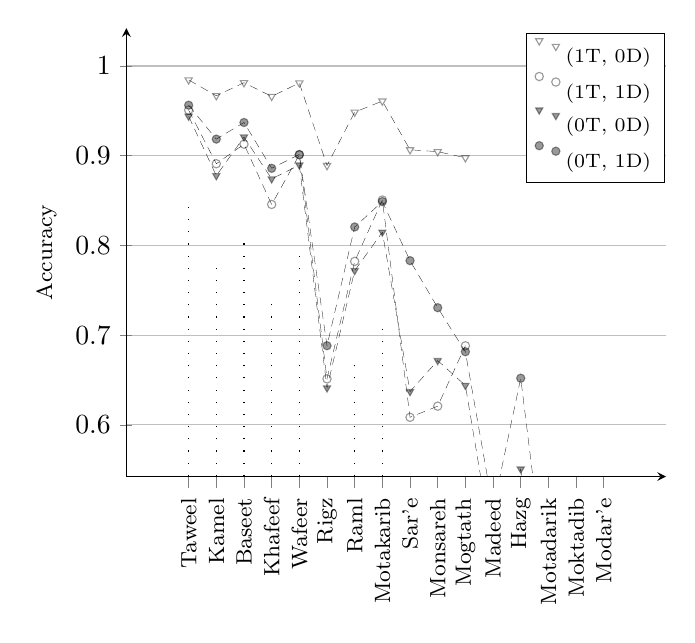
\begin{tikzpicture}[scale=1]
  \begin{axis}[
    axis x line = bottom,
    axis y line = left,
    ymajorgrids = true,
    ybar,
    enlargelimits=0.15,
    legend style={at={(0.87,0.99)},
      anchor=north,legend columns=1},
    ylabel={Accuracy},
    ylabel style = {font=\footnotesize},
    symbolic x coords={Taweel, Kamel, Baseet, Khafeef, Wafeer, Rigz, Raml, Motakarib, Sar'e, Monsareh, Mogtath, Madeed, Hazg, Motadarik, Moktadib, Modar'e},
    xtick=data,
    xticklabel style = {font=\footnotesize},
    nodes near coords align={vertical},
    x tick label style={rotate=90, anchor=east},
    bar width=2pt,
    ymin=0.6,
    ]

    % trimmed no-diacritic (Empty Triangle)
    \addplot[mark=triangle, every mark/.append style={rotate=180},
    thin, only marks, mark size=1.5pt, point meta=explicit symbolic, opacity=0.4]
    coordinates {
      % (1T, 0D)
      (Wafeer,    0.9811213222198475)       
      (Monsareh,  0.9045746962115797)       
      (Mogtath,   0.897708216880939 )       
      (Motakarib, 0.9609120521172638)       
      (Kamel,     0.966898378020523 )       
      (Taweel,    0.9844991757498216)       
      (Sar'e,     0.9066397034041119)       
      (Raml,      0.9485771342985522)       
      (Rigz,      0.8889925373134329)       
      (Khafeef,   0.9661488673139158)       
      (Baseet,    0.9814341393906374) 
      (Madeed,     0)  
      (Hazg,       0) (Motadarik,  0) 
      (Moktadib,   0) 
      (Modar'e,    0)
    };

    % trimmed diacritic (Empty Circle)
    % (1T, 1D)
    \addplot[mark=o, thin, only marks, mark size=1.5pt, point
    meta=explicit symbolic, opacity=0.4]
    coordinates{
      (Wafeer,     0.9009759920210871)
      (Monsareh,   0.6208005718370264)
      (Mogtath,    0.6880939072107323)
      (Motakarib,  0.8506281991624011)
      (Kamel,      0.8910956636875207)
      (Taweel,     0.9508402430922914)
      (Sar'e,      0.6083586113919784)
      (Raml,       0.7822016974538193)
      (Rigz,       0.6512042062415196)
      (Khafeef,    0.8456957928802589)
      (Baseet,     0.9128703742508696)
    };


    % full no-diacritic (Full Triangle)
    % (0T, 0D)
    \addplot[mark=triangle*, every mark/.append style={rotate=180},
    thin, only marks, mark size=1.5pt, point meta=explicit symbolic, opacity=0.4]
    coordinates {
      (Wafeer,    0.889584964761159)
      (Monsareh,  0.6716101694915254)
      (Madeed,    0.45979899497487436)
      (Mogtath,   0.6439135381114903)
      (Motakarib, 0.8148088917319687)
      (Kamel,     0.8776972469479428)
      (Taweel,    0.9439529481540059)
      (Sar'e,     0.6370179948586119)
      (Raml,      0.7719209325899645)
      (Rigz,      0.64107517849643)
      (Khafeef,   0.8741908607319105)
      (Baseet,    0.9208657001620072)
      (Moktadib,  0.16326530612244897)
      (Hazg,      0.5506493506493506)
      (Modar'e,   0.0)
      (Motadarik, 0.28)
    };

    % full diacritic (Full Circle)
    % (0T, 1D)
    \addplot[mark=*, thin, only marks, mark size=1.5pt, point
    meta=explicit symbolic, opacity=0.4]
    coordinates {
      (Wafeer,    0.9014024346835623)
      (Monsareh,  0.7305790960451978)
      (Madeed,    0.5062814070351759)
      (Mogtath,   0.6814562002275313)
      (Motakarib, 0.8488725411802335)
      (Kamel,     0.9185383195083638)
      (Taweel,    0.9563337122522612)
      (Sar'e,     0.7830334190231363)
      (Raml,      0.8205778003041054)
      (Rigz,      0.6881982360352793)
      (Khafeef,   0.8859834647183235)
      (Baseet,    0.9370664229634861)
      (Moktadib,  0.3673469387755102)
      (Hazg,      0.6519480519480519)
      (Modar'e,   0.08333333333333333)
      (Motadarik, 0.40190476190476193)
    };

    \legend{
      {\scriptsize (1T, 0D)},
      {\scriptsize (1T, 1D)},
      {\scriptsize (0T, 0D)},
      {\scriptsize (0T, 1D)},
    }

    % Dotted line
    \draw[loosely dotted] (axis cs:Wafeer,    0) -- (axis cs:Wafeer,     0.789584964761159);
    \draw[loosely dotted] (axis cs:Monsareh,  0) -- (axis cs:Monsareh,   0.5208005718370264);
    \draw[loosely dotted] (axis cs:Mogtath,   0) -- (axis cs:Mogtath,    0);
    \draw[loosely dotted] (axis cs:Motakarib, 0) -- (axis cs:Motakarib,  0.7148088917319687);
    \draw[loosely dotted] (axis cs:Kamel,     0) -- (axis cs:Kamel,      0.7776972469479428);
    \draw[loosely dotted] (axis cs:Taweel,    0) -- (axis cs:Taweel,     0.8439529481540059);
    \draw[loosely dotted] (axis cs:Sar'e,     0) -- (axis cs:Sar'e,      0.5083586113919784);
    \draw[loosely dotted] (axis cs:Raml,      0) -- (axis cs:Raml,       0.6719209325899645);
    \draw[loosely dotted] (axis cs:Rigz,      0) -- (axis cs:Rigz,       0.54107517849643);
    \draw[loosely dotted] (axis cs:Khafeef,   0) -- (axis cs:Khafeef,    0.7456957928802589);
    \draw[loosely dotted] (axis cs:Baseet,    0) -- (axis cs:Baseet,     0.8128703742508696);
    \draw[loosely dotted] (axis cs:Moktadib,  0) -- (axis cs:Moktadib,   0);
    \draw[loosely dotted] (axis cs:Madeed,    0) -- (axis cs:Madeed,     0.35979899497487436);
    \draw[loosely dotted] (axis cs:Hazg,      0) -- (axis cs:Hazg,       0.4506493506493506);
    \draw[loosely dotted] (axis cs:Modar'e,   0) -- (axis cs:Modar'e,    0);
    \draw[loosely dotted] (axis cs:Motadarik, 0) -- (axis cs:Motadarik,  0.18);


    % connecting  models accuracies

    % Empty Triangle
    % (1T, 0D)
    \draw[line width=0.1pt, densely dashed]
    (axis cs:Taweel,        0.9844991757498216)
    -- (axis cs:Kamel,      0.966898378020523 )
    -- (axis cs:Baseet,     0.9814341393906374)
    -- (axis cs:Khafeef,    0.9661488673139158)
    -- (axis cs:Wafeer,     0.9811213222198475)
    -- (axis cs:Rigz,       0.8889925373134329)
    -- (axis cs:Raml,       0.9485771342985522)
    -- (axis cs:Motakarib,  0.9609120521172638)
    -- (axis cs:Sar'e,      0.9066397034041119)
    -- (axis cs:Monsareh,   0.9045746962115797)
    -- (axis cs:Mogtath,    0.897708216880939 );

   % Empty Circle
   % (1T, 1D)
   \draw[line width=0.1pt, densely dashed]
   (axis cs:Taweel,        0.9508402430922914)
   -- (axis cs:Kamel,      0.8910956636875207)
   -- (axis cs:Baseet,     0.9128703742508696)
   -- (axis cs:Khafeef,    0.8456957928802589)
   -- (axis cs:Wafeer,     0.9009759920210871)
   -- (axis cs:Rigz,       0.6512042062415196)
   -- (axis cs:Raml,       0.7822016974538193)
   -- (axis cs:Motakarib,  0.8506281991624011)
   -- (axis cs:Sar'e,      0.6083586113919784)
   -- (axis cs:Monsareh,   0.6208005718370264)
   -- (axis cs:Mogtath,    0.6880939072107323);


    % Full Triangle
    % (0T, 0D)
    \draw[line width=0.1pt, densely dashed]
    (axis cs:Taweel,        0.9439529481540059)
    -- (axis cs:Kamel,      0.8776972469479428)
    -- (axis cs:Baseet,     0.9208657001620072)
    -- (axis cs:Khafeef,    0.8741908607319105)
    -- (axis cs:Wafeer,     0.889584964761159)
    -- (axis cs:Rigz,       0.64107517849643)
    -- (axis cs:Raml,       0.7719209325899645)
    -- (axis cs:Motakarib,  0.8148088917319687)
    -- (axis cs:Sar'e,      0.6370179948586119)
    -- (axis cs:Monsareh,   0.6716101694915254)
    -- (axis cs:Mogtath,    0.6439135381114903)
    -- (axis cs:Madeed,     0.4597989949748743)
    -- (axis cs:Hazg,       0.5506493506493506)
    -- (axis cs:Motadarik,  0.28)
    -- (axis cs:Moktadib,   0.1632653061224489)
    -- (axis cs:Modar'e,    0.0               );


   % Full Circle
   % (0T, 1D)
   \draw[line width=0.1pt, densely dashed]
   (axis cs:Taweel,        0.9563337122522612)
   -- (axis cs:Kamel,      0.9185383195083638)
   -- (axis cs:Baseet,     0.9370664229634861)
   -- (axis cs:Khafeef,    0.8859834647183235)
   -- (axis cs:Wafeer,     0.9014024346835623)
   -- (axis cs:Rigz,       0.6881982360352793)
   -- (axis cs:Raml,       0.8205778003041054)
   -- (axis cs:Motakarib,  0.8488725411802335)
   -- (axis cs:Sar'e,      0.7830334190231363)
   -- (axis cs:Monsareh,   0.7305790960451978)
   -- (axis cs:Mogtath,    0.6814562002275313)
   -- (axis cs:Madeed,     0.5062814070351759)
   -- (axis cs:Hazg,       0.6519480519480519)
   -- (axis cs:Motadarik,  0.4019047619047619)
   -- (axis cs:Moktadib,   0.3673469387755102)
   -- (axis cs:Modar'e,    0.0833333333333333);

  \end{axis}
\end{tikzpicture}

  \caption{The per-class accuracy for the best four models: \{\text{0T},\ \text{1T}\} $\times$
    \{\text{0D},\ \text{1D}\}; the $x$-axis is sorted by class size as in
    Figure~\ref{fig:footn-footn-class}. There is a descending trend with the class size, with the
    exception at \textit{Rigz} meter.}\label{fig:footn-both-models}
\end{figure}
Next, we investigate the per-class accuracy. For each of the four combinations of
\textit{trimming} $\times$ \textit{diacritic}, we select the best accuracy out of the three possible
encodings. From Figure~\ref{fig:ArabicModelsResults}, it is clear that all of them will be at TwoE,
except (1T, 0D, BinE), which is the best overall model as discussed above.

Figure~\ref{fig:footn-both-models} displays the per-class accuracy of these four models. The class
names (meters) are ordered on the $x$-axis according to their individual class size (the same order
of Figure~\ref{fig:footn-footn-class}). Several comments are in order. The overall accuracy of each of
the four models is around 0.95 (Figure~\ref{fig:ArabicModelsResults}); however, for the four models
the per-class accuracy of only 6 classes is around this value. For some classes the accuracy drops
significantly. Moreover, the common trend for the four models is that the per-class accuracy
decreases with the class size for the first 11 classes. Then, the accuracy of the two models with
\textit{trimming} keeps decreasing significantly for the remaining 5 classes. Although this
trend is associated with class size, this could only be correlations without causation. This
phenomenon, along with what was concluded above for the inconsistent effect of loss
\textit{weighting}, emphasize the importance of a more prudent design of the \textit{weighting}
function. In addition, the same full set of experiments can be re-conducted with enforcing all
classes to have equal size to assert/negate the causality assumption (Sec.~\ref{sec:discussion}).

\bigskip

\subsubsection{Encoding Effect on Learning rate and Memory
  Utilization}\label{sec:learning-rate-memory}
\begin{figure}[!tb]
  \centering
  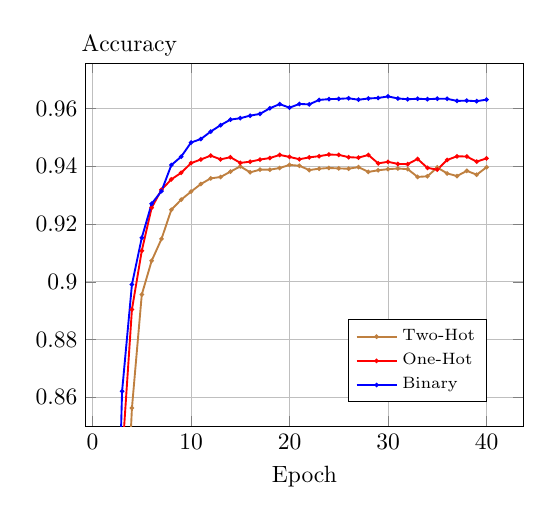
\begin{tikzpicture}[scale=0.85]
    \begin{axis}[
  height=7cm,
  grid=major,
  every axis y label/.style= {at={( 0.1, 1.1)}, anchor=north},
  xlabel={Epoch},
  ylabel={Accuracy},
  legend style={at={(0.6, 0.18)},anchor=west},
  every axis legend/.append style={nodes={right}},
  ymin = 0.85,
  name=left plot,
  title style={at={(0.5,-.4)}}
  ]



  \addplot[color=brown, mark=*, thick, mark size=0.5pt] coordinates {

    % twohot
    (1  , 0.4973408579826355)
    (2  , 0.6637325882911682)
    (3  , 0.7843776345252991)
    (4  , 0.8562803268432617)
    (5  , 0.8955804109573364)
    (6  , 0.9072529673576355)
    (7  , 0.9148279428482056)
    (8  , 0.9249432682991028)
    (9  , 0.9284470081329346)
    (10 , 0.9312249422073364)
    (11 , 0.9338576793670654)
    (12 , 0.9358240365982056)
    (13 , 0.9362859129905701)
    (14 , 0.9381598234176636)
    (15 , 0.9399744272232056)
    (16 , 0.9379156827926636)
    (17 , 0.9388328790664673)
    (18 , 0.9388262629508972)
    (19 , 0.939400315284729)
    (20 , 0.9404956698417664)
    (21 , 0.9401789307594299)
    (22 , 0.9387009143829346)
    (23 , 0.9391694068908691)
    (24 , 0.9394267201423645)
    (25 , 0.939261794090271)
    (26 , 0.9391694068908691)
    (27 , 0.9397236704826355)
    (28 , 0.9380608797073364)
    (29 , 0.9386216998100281)
    (30 , 0.9390044212341309)
    (31 , 0.9392420053482056)
    (32 , 0.9390110373497009)
    (33 , 0.9363254904747009)
    (34 , 0.9365366101264954)
    (35 , 0.9395982623100281)
    (36 , 0.9375395774841309)
    (37 , 0.9366289973258972)
    (38 , 0.9384303689002991)
    (39 , 0.9370908737182617)
    (40 , 0.9396642446517944)
  };





  \addplot[color=red, mark=*, thick, mark size=0.5pt] coordinates {
    % onehot
    (1  , 0.5241501331329346)
    (2  , 0.6912611126899719)
    (3  , 0.8391179442405701)
    (4  , 0.8904072642326355)
    (5  , 0.9107500910758972)
    (6  , 0.9256294965744019)
    (7  , 0.9318781495094299)
    (8  , 0.9354742765426636)
    (9  , 0.9377507567405701)
    (10 , 0.9410961270332336)
    (11 , 0.9423761963844299)
    (12 , 0.9436959028244019)
    (13 , 0.9424092173576355)
    (14 , 0.9431548118591309)
    (15 , 0.9411951303482056)
    (16 , 0.9415910243988037)
    (17 , 0.942330002784729)
    (18 , 0.9428513050079346)
    (19 , 0.9439400434494019)
    (20 , 0.9432538151741028)
    (21 , 0.9424421787261963)
    (22 , 0.9430954456329346)
    (23 , 0.9435111284255981)
    (24 , 0.9440720081329346)
    (25 , 0.9439598321914673)
    (26 , 0.9431614279747009)
    (27 , 0.9429964423179626)
    (28 , 0.9439268112182617)
    (29 , 0.9410235285758972)
    (30 , 0.9415580034255981)
    (31 , 0.9408321976661682)
    (32 , 0.9407595992088318)
    (33 , 0.9425477981567383)
    (34 , 0.939453125)
    (35 , 0.9388592839241028)
    (36 , 0.942191481590271)
    (37 , 0.9434715509414673)
    (38 , 0.9433857798576355)
    (39 , 0.9416041970252991)
    (40 , 0.9427457451820374)
  };




  \addplot[color=blue, mark=*, thick, mark size=0.5pt] coordinates {
    % binary
    (1  , 0.4176618158817291)
    (2  , 0.7385522127151489)
    (3  , 0.8620811104774475)
    (4  , 0.8990639448165894)
    (5  , 0.9152568578720093)
    (6  , 0.9270322322845459)
    (7  , 0.9314031600952148)
    (8  , 0.9404243230819702)
    (9  , 0.9433448910713196)
    (10 , 0.9482346773147583)
    (11 , 0.9494454860687256)
    (12 , 0.9520400762557983)
    (13 , 0.9542421698570251)
    (14 , 0.956171452999115)
    (15 , 0.9566637873649597)
    (16 , 0.9575485587120056)
    (17 , 0.9581539630889893)
    (18 , 0.9601032733917236)
    (19 , 0.9615402817726135)
    (20 , 0.9603028297424316)
    (21 , 0.9616068005561829)
    (22 , 0.9614471197128296)
    (23 , 0.9629971981048584)
    (24 , 0.9632699489593506)
    (25 , 0.9633697867393494)
    (26 , 0.9635560512542725)
    (27 , 0.9630637168884277)
    (28 , 0.9634895324707031)
    (29 , 0.9636757969856262)
    (30 , 0.9642080068588257)
    (31 , 0.963502824306488)
    (32 , 0.9632300734519958)
    (33 , 0.9634096622467041)
    (34 , 0.9632500410079956)
    (35 , 0.963416337966919)
    (36 , 0.9633830785751343)
    (37 , 0.962651252746582)
    (38 , 0.962751030921936)
    (39 , 0.9625581502914429)
    (40 , 0.9630969762802124)
  };



  \legend{
    {\scriptsize Two-Hot},
    {\scriptsize One-Hot},
    {\scriptsize Binary},
  }

\end{axis}

  \end{tikzpicture}
  \caption{Encoding effect on learning rate of the best model configurations (1T, 0D, 4L, 82U, 0W)
    with each of the three encodings.}~\label{fig:ConvergenceMemory}
\end{figure}
Figure~\ref{fig:ConvergenceMemory}-a shows the learning curve of the best model (4L, 82U, 0W, 1T,
0D, BinE), which converges to 0.9638, the same value displayed on
Figure~\ref{fig:ArabicModelsResults}. The Figure displays, as well, the learning curve of the same
model and parameters but with using the other two encodings. The Figure shows no big difference in
convergence speed among different encodings.


\subsection{Results of English Dataset}\label{sec:english-results}
The result presentation and interpretation for the experiments on English dataset are much easier
because of the absence of \textit{diacritic}, \textit{trimming}, and loss \textit{weighting}
parameters. The relative size of the two datasets has to be brought to attention; from
Figure~\ref{fig:footn-footn-class}, there is almost a factor of 100 in favor of the Arabic dataset.

\bigskip

\subsubsection{Overall Accuracy}\label{sec:overall-accuracy}
\begin{figure}[!tb]
  \centering
  \begin{tikzpicture}[scale=0.8]
    \begin{axis}[
  major x tick style = transparent,
  height=7cm,
  legend style={at={(0.7, 0.2)},anchor=west},
  every axis legend/.append style={nodes={right}},
  name=left plot,
  xtick distance=1,
  axis x line = bottom,
  axis y line = left,
  xmin=0,
  xmax=3.5,
  x=1.5cm,
  title={\small (a) \textit{Overall accuracy}},
  title style={at={(0.5,-.4)}},
  xticklabels = {, ,},
  ymajorgrids = true,
  nodes near coords,
  ylabel = {Accuracy},
  ylabel style = {font=\footnotesize},
  ymin=0.72,
  ymax=0.857,
  ]



  % Symbols of column 1 (the binary)
  \addplot[pointBiGRU=blue] coordinates {
(1, 0.8169014084507042) %tr-Experiment62 BiGRU

  };
  \addplot[pointGRU=blue] coordinates {
(1, 0.7859154929577463) %tr-Experiment57 GRU
  };
  \addplot[pointLSTM=blue] coordinates {
(1, 0.7690140845070422) %tr-Experiment53 LSTM

  };
  \addplot[pointBiLSTM=blue] coordinates {
(1, 0.7661971830985915) %tr-Experiment72 BiLSTM

  };

  % Symbols of column 2 (the one hot)
  \addplot[pointBiGRU=red] coordinates {
    (2, 0.8264788732394366) %tr-Experiment29 BiGRU

  };
  \addplot[pointGRU=red] coordinates {
(2, 0.8214084507042254) %tr-Experiment24 GRU

  };
  \addplot[pointLSTM=red] coordinates {
(2, 0.8022535211267606) %tr-Experiment17 LSTM

  };
  \addplot[pointBiLSTM=red] coordinates {
(2, 0.7650704225352113) %tr-Experiment36 BiLSTM

  };

  % Binary
  \addplot[pointModelsFiguresStyle=blue, mark size=0.7pt, mark=-]
  coordinates {
(1, 0.7138028169014086) %tr-Experiment68
(1, 0.7211267605633802) %tr-Experiment41
(1, 0.7245070422535211) %tr-Experiment71
(1, 0.7256338028169014) %tr-Experiment69
(1, 0.7278873239436621) %tr-Experiment45
(1, 0.7312676056338029) %tr-Experiment70
(1, 0.7357746478873239) %tr-Experiment39
(1, 0.7380281690140845) %tr-Experiment67
(1, 0.7414084507042253) %tr-Experiment40
(1, 0.7425352112676056) %tr-Experiment44
(1, 0.7447887323943663) %tr-Experiment42
(1, 0.7447887323943663) %tr-Experiment47
(1, 0.7498591549295774) %tr-Experiment51
(1, 0.7526760563380281) %tr-Experiment49
(1, 0.7543661971830986) %tr-Experiment43
(1, 0.7571830985915493) %tr-Experiment50
(1, 0.7588732394366198) %tr-Experiment48
(1, 0.7622535211267607) %tr-Experiment38
(1, 0.7650704225352112) %tr-Experiment54
(1, 0.7661971830985915) %tr-Experiment72
(1, 0.7661971830985916) %tr-Experiment46
(1, 0.7684507042253521) %tr-Experiment52
(1, 0.7690140845070422) %tr-Experiment53
(1, 0.7735211267605634) %tr-Experiment56
(1, 0.7752112676056337) %tr-Experiment60
(1, 0.7780281690140846) %tr-Experiment55
(1, 0.7808450704225353) %tr-Experiment59
(1, 0.7825352112676058) %tr-Experiment58
(1, 0.7859154929577463) %tr-Experiment57
(1, 0.7870422535211268) %tr-Experiment37
(1, 0.7954929577464789) %tr-Experiment64
(1, 0.7988732394366197) %tr-Experiment66
(1, 0.8011267605633803) %tr-Experiment63
(1, 0.8022535211267606) %tr-Experiment65
(1, 0.8050704225352113) %tr-Experiment61
(1, 0.8169014084507042) %tr-Experiment62
  };
  % OneHot
  \addplot[pointModelsFiguresStyle=red, mark size=0.7pt, mark=-]
  coordinates {
(2, 0.7059154929577465) % tr-Experiment32
(2, 0.716056338028169)  % tr-Experiment31
(2, 0.7295774647887323) % tr-Experiment4
(2, 0.7307042253521127) % tr-Experiment33
(2, 0.7329577464788732) % tr-Experiment10
(2, 0.7340845070422535) % tr-Experiment14
(2, 0.7374647887323944) % tr-Experiment9
(2, 0.7380281690140844) % tr-Experiment7
(2, 0.7459154929577465) % tr-Experiment34
(2, 0.755492957746479)  % tr-Experiment35
(2, 0.7583098591549295) % tr-Experiment3
(2, 0.7594366197183099) % tr-Experiment2
(2, 0.7616901408450705) % tr-Experiment13
(2, 0.7622535211267606) % tr-Experiment16
(2, 0.7628169014084507) % tr-Experiment15
(2, 0.763943661971831)  % tr-Experiment8
(2, 0.7650704225352113) % tr-Experiment36
(2, 0.7684507042253521) % tr-Experiment5
(2, 0.779718309859155)  % tr-Experiment6
(2, 0.7808450704225353) % tr-Experiment12
(2, 0.7836619718309861) % tr-Experiment11
(2, 0.7904225352112677) % tr-Experiment21
(2, 0.8005633802816902) % tr-Experiment1
(2, 0.8011267605633803) % tr-Experiment19
(2, 0.8022535211267606) % tr-Experiment17
(2, 0.8045070422535211) % tr-Experiment23
(2, 0.8090140845070422) % tr-Experiment20
(2, 0.8107042253521127) % tr-Experiment26
(2, 0.811830985915493)  % tr-Experiment28
(2, 0.8129577464788732) % tr-Experiment25
(2, 0.815774647887324)  % tr-Experiment18
(2, 0.816338028169014)  % tr-Experiment22
(2, 0.8174647887323944) % tr-Experiment27
(2, 0.8180281690140845) % tr-Experiment30
(2, 0.8214084507042254) % tr-Experiment24
(2, 0.8264788732394366) % tr-Experiment29
  };


    \addplot[pointBiLSTM=black] coordinates {(1, 0)};\label{BiLSTM}
    \addplot[pointLSTM=black]   coordinates {(1, 0)};\label{LSTM}
    \addplot[pointBiGRU=black]  coordinates {(1, 0)};\label{BiGRU}
    \addplot[pointGRU=black]    coordinates {(1, 0)};\label{GRU}
    \addplot[pointRug=red]      coordinates {(1, 0)};\label{OneHot}
    \addplot[pointRug=blue]     coordinates {(1, 0)};\label{Binary}
\end{axis}

    % Cells legend
    \node [draw,fill=white] at (4.3,1.2) {\shortstack[l]{
    \ref{BiGRU} \scriptsize{BiGRU}\\
    \ref{GRU} \scriptsize{GRU}\\
    \ref{LSTM} \scriptsize{LSTM}\\
    \ref{BiLSTM} \scriptsize{BiLSTM}
    }};

    % Encoding legend
    \node [draw,fill=white] at (2.6,-0.9) {\shortstack[l]{
    \ref{Binary} \scriptsize{\scriptsize{Binary(BinE)}}
    \ref{OneHot} \scriptsize{\scriptsize{One-Hot(OneE)}}
    }};

\node at (7.5 * 0.2, 5.2) {\scriptsize 7L};
\node at (7.5 * 0.2, 5.2 -0.3) {\scriptsize 40U};

\node at (15 * 0.2, 5.2) {\scriptsize 4L};
\node at (15 * 0.2, 5.2 -0.3) {\scriptsize 40U};

    \begin{axis}[
  symbolic x coords={Iambic,Trochaic,Anapaestic,Dactyl},
  xtick=data,
  every axis y label/.style= {at={( 0.1, 1.1)}, anchor=north},
  x tick label style={font=\footnotesize},
  height=7cm,
  x=0.5cm,
  ylabel={Accuracy},
  enlarge x limits=0.3,
  enlarge y limits=0.07,
  x tick label style={rotate=90, anchor=east},
  /pgf/bar width=20pt,
  at={($(left plot.south east)+(1.5cm,0)$)},
  title={\small (b) \textit{Per-class Accuracy}},
  title style={at={(0.5,-.4)}}
  ]

    \addplot[mark=triangle*, every mark/.append style={rotate=180},
thin, only marks, mark size=1.5pt, point meta=explicit symbolic, opacity=0.4]
   coordinates {
    % Ordering does not effect.
      (Iambic,     0.9099264705882353)
      (Anapaestic, 0.9788732394366197)
      (Trochaic,   0.8827977315689981)
      (Dactyl,     0.6535714285714286)
    };

  \draw[line width=0.1pt, densely dashed]
      (axis cs:Iambic,       0.9099264705882353)
   -- (axis cs:Trochaic,     0.8827977315689981 )
   -- (axis cs:Anapaestic,   0.9788732394366197)
   -- (axis cs:Dactyl,       0.6535714285714286);


\end{axis}

  \end{tikzpicture}
  \caption{Accuracy of experiments on English dataset. (a) Overall accuracy of the 192
    experiments plotted as 2 vertical rug plots (one at each data representation: \{OneE, BinE\});
    each represents 96 exp. (for network configurations: \{3L, 4L, 5L, 6L, 7L, 8L\} $\times$ \{30U,
    40U, 50U, 60U\} $\times$ \{LSTM,\ BiLSTM,\ GRU,\ BiGRU\}). For each rug plot the best model of each
    of the four cell types---(Bi-)LSTM and (Bi-)GRU---is labeled differently. Consistently, the BiGRU
    was the winner, and its network configuration parameters are listed at the top of each rug
    plot. (b) The per-class accuracy for the best model of the 192 experiments; the $x$-axis is
    sort by the class size as in Figure~\ref{fig:footn-footn-class}. No particular trend with the
    class size is observed.}~\label{english_results}
\end{figure}

Similar to Figure~\ref{fig:ArabicModelsResults}, Figure~\ref{english_results}-a displays the accuracy of 96 network configurations ($y$-axis) for each of the 2 dataset representations
($x$-axis). The Figure shows that the highest accuracy, 0.8265, is obtained using (4L, 40U,
OneE), and BiGRU network. The \textit{encoding} is the only parameter for data representation. OneE
achieves higher accuracy than, but close to, BinE. Once again, we anticipate that experimenting
with more network configuration should resolve this difference (Sec.~\ref{sec:discussion}).

For Network configuration parameters, we start with the \textit{cell} type. At each encoding, the
best accuracy of each \textit{cell} type in descending order is: BiGRU, GRU, LSTM, then
BiLSTM\@. (Bi-)GRU models may by more suitable for this smaller size dataset. For \textit{layers},
the best models on OneE was 3L and on BinE was 7L. In contrast to the Arabic dataset, the simple 4L
achieved a better accuracy than the complex 7L, with no clear effect of cell \textit{size}. (More
discussion on that in Sec.~\ref{sec:discussion}).

\bigskip

\subsubsection{Per-Class (Meter) Accuracy}\label{sec:per-class-meter}
Figure~\ref{english_results}-b is a per-class accuracy for the best model (4L, 40U, OneE, BiGRU);
the meters are ordered on the $x$-axis descendingly with the class size as in
Figure~\ref{fig:footn-footn-class}-b. It is clear that class size is not correlated with
accuracy. Even for the smallest class, Dactyl, its size is almost one third the Iambic class
(Figure~\ref{fig:footn-footn-class}-b), which is not a huge skewing factor. A more reasonable
interpretation is this. Dactyl meter is pentameter or more; while other meters have less
repetitions. This makes Dactyl verses very distant in character space from others. And since the
network will train to optimize the overall accuracy, this may be on the expense on the class that is
both small in size and setting distant in feature space from others. (More discussion on that in
Sec.~\ref{sec:discussion}).
